\documentclass[conference]{IEEEtran}
\IEEEoverridecommandlockouts


\usepackage[pdftex]{graphicx}
\usepackage{amsmath,amssymb,amsfonts}
\usepackage{algorithmic}
\usepackage{graphicx}
\usepackage{float}
\usepackage{comment}
\usepackage{textcomp}
\usepackage{xcolor}
\usepackage{hyperref}
\usepackage[style=ieee]{biblatex}
\addbibresource{paper.bib}
\usepackage{url}

% correct bad hyphenation here
\hyphenation{op-tical net-works semi-conduc-tor}

\newcommand{\todo}[1]{{\color{olive} TODO: #1}}

% Regler ti skrivning: 
% 1. Altid nutid
% 2. Brug 1. persons flertal stedord (We/us/our/ours)
% 3. Skriv formelt og uden sammentrækninger (don't do this) 
% 

\begin{document}

\title{Telemetry Module for Solar Vehicle}

\author{\IEEEauthorblockN{Victor Alexander Hansen s194027, Steffan Martin Kunoy s194006, Tjark Petersen, s186083}
\IEEEauthorblockA{\textit{Department of Electrical Engineering} \\
\textit{Technical Uniservity of Denmark}\\
Kgs. Lyngby, Denmark \\
31015 Introductory project - electrotechnology\\
s194027@student.dtu.dk, s194006@student.dtu.dk, s186083@student.dtu.dk}}
%\author{Victor Alexander Hansen, Steffan Martin Kunoy, Tjark Petersen}

\maketitle

% As a general rule, do not put math, special symbols or citations
% in the abstract or keywords.
\begin{abstract}
Abstract
\end{abstract}

% Note that keywords are not normally used for peerreview papers.
\begin{IEEEkeywords}
ROAST, telemetry, CAN
\end{IEEEkeywords}



\section{Introduction}

\IEEEPARstart{I}{n} 2023, the DTU Roadrunners Solar Team (abbreviated ROAST) is set to participate in the Bridgestone World Solar Challenge, a race spanning over 3000 km across Australia from Darwin in the Northern Territory to Adelaide in South Australia. The solar car has limited opportunities for recharging during the race, so its the main energy source will be the sun. To this end, solar panels will cover the car, however, the solar car is only allowed to have a maximum of 4 square meters of solar panels. This emphasizes the need to create an energy-efficient solar car to win the race \cite{wsc}.

Throughout the race the solar car will be monitored by a support vehicle, which can monitor the car's condition and should be able to issue commands to the solar cars internal systems. This is a crucial function as the solar car will be navigating Australia's busy highways, where the heat and tire pressure may cause a detriment to the vehicle. The support vehicle will therefore be able to analyze and react to the data stream being transmitted from the solar car, even when the driver is preoccupied with driving the car. 

Additionally, valuable data can be collected during the race which can help to identify possible areas of improvement of the solar car. Therefore a "black box" system is needed to capture all system activity in a local storage.

These key functionalities require a system which is able to read and write data from the solar cars on-board CAN (Controller Area Network) bus and transmit it via an RF-transceiver to the support vehicle, while simultaneously logging data locally. The support vehicle is equipped with a similar module such that the support crew can react to the data manually or automatically by sending commands back to the CAN bus via RF. Thus, the capabilities of such a telemetry module play a vital role in the communication between both vehicles, considering that the distance between them may be up to 1 km depending on traffic conditions.

The telemetry system must both serve the purpose of fulfilling the necessary specifications for communication, while also being as energy-efficient as possible. This project aims at implementing a functioning prototype for a telemetry system while mainly focusing on the former of the two objectives, that is, ensuring that the system meets the specifications with a solid solution.

This paper begins with giving a more precise problem statement and introducing the methodology used throughout the project. Thereafter, the design... \todo{Skal laves når strukturen er slået fast}

\subsection{Problem Statement}
Remote sensing of data from the solar car will give the ROAST team a competitive advantage as the support vehicle will be able to take on a more active role in managing and optimising the car's performance. This will ease the burden on the driver and leverage the expertise of the supporting crew. For these reasons we have chosen to focus our project on the following points:
\begin{itemize}
    \item How can we design a module that can read and write sensor data and commands from a CAN bus network? 
    \item How can CAN data be transmitted securely over a distance of up to one kilometer?
    \item How does the support-car module process data upon receiving it from the solar car?
    \item What is the best method for storing data locally (black box) while being accessible at a later time?
    \item How can the CAN data be made accessible in the support vehicle for further processing e.g. in Matlab?
\end{itemize}

\section{Methodology}
The project methodology has largely consisted of making a preliminary design to be completed in a series of design sprints. At first a detailed specification was drafted which then served as a reevaluation tool and an overall guidance each time a sprint was completed and when the goal for the next sprint had to be selected. Using the specification, we made a prototype setup of the hardware on breadboards as our first sprint. The following sprints would then mostly have software development objectives, such as achieving a first transmission and receiving of data. Finally, a last hardware sprint was conducted where we soldered our hardware to a perf board.

During the development of the software functions, we also verified and validated our code design. In verification the code and its functionality was discussed. To validate our code we made unit tests that test the actual behaviour of our code against the intended behaviour.

During the software development phase, we attempted to make our debugging more efficient with the use of a debugger. However, this proved quite troublesome, as the Teensy 3.6 board does not have an on-board debugger and in general is not very suited for debuggers. If we had insisted on using a debugger such as st-link, we would have had to hold or solder wires to the debug ports on the Teensy board's backside, which would complicate our prototype setup. Therefore, we decided not to spent more time on finding a debugger solution. This was a clear setback, as debugging could only be conducted by sending text over the serial connection.

\section{Design}
The overall system consists of three separate modules; the Solar Car Unit which communicates with the Support Vehicle Unit via a wireless RF connection, which in turn interacts with the Support Vehicle Laptop through a serial USB connection. The schematic for the system is outlined in Figure \ref{fig:schematic}. 
\begin{figure}[H]
    \centering
    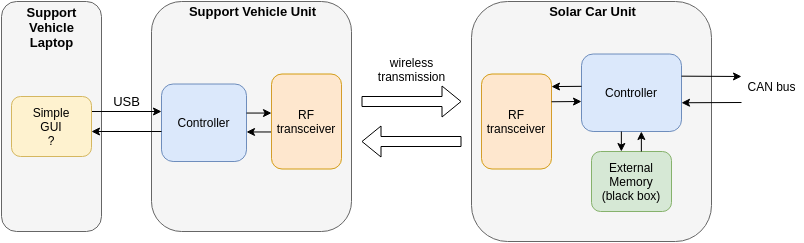
\includegraphics[width=0.5\textwidth]{documentation/images/schematic.png}
    \caption{Overview of the system's components in block diagram form.}
    \label{fig:schematic}
\end{figure}

\section{Components}
\subsection{CAN bus}
% MCP
\subsection{RF network} % Steffan
The system uses two nRF24L01+ transceivers to provide a bidirectional connection between the Solar Car and Support Vehicle over the 2.4 GHz ISM band. The module features a detachable antenna, power amplifier and low-noise amplifier to provide a theoretical range in excess of 1000 m at data rates of up to 2 Mbit/s.

An advantage of using an off-the-shelf RF module is the automated message protocol, known as Enhanced Shockburst$^{\copyright}$.

The nRF24L01+ module uses the Enhanced Shockburst $\copyright$ packet structure to transmit messages over the 2.4 GHz ISM band. Messages contain a data payload of up to 32 bytes, allowing us comfortably to transmit one CAN telemetry message per packet \cite{shockburst}. Further, the package structure includes a preamble, address, packet and CRC bytes segments as shown in Figure \ref{fig:shockburst}. 

\begin{figure}[h]
    \centering
    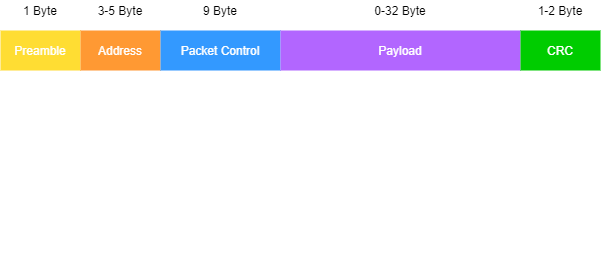
\includegraphics[width=0.5\textwidth]{documentation/images/EnhancedShockburst.png}
    \caption{The Enhanced Shockburst $\copyright$ packet structure.}
    \label{fig:shockburst}
\end{figure}

\subsection{SD card}
\subsection{Microcontrollers} % Steffan

\section{Software Stack}

Several of the key functionalities of the telemetry are implemented in software. This together with the aim of designing a system which is easy to extend in the future makes the choice of software frameworks very important, since they affect reusability and maintainability of the developed code.

\subsection{Build system}
As a build system, platformIO \cite{platformIO} was chosen for the project. It is a version control friendly, cross-platform embedded build tool which includes library management and works by defining \textit{environments} to allow development with different embedded platforms on the same code base. Other project groups working on the solar car in parallel integrated their software into the platformIO ecosystem as well, making extensive code reuse in the future possible.

\subsection{Real Time Operating System}
We chose to build the software for the telemetry system on top of a real time operating system. The small kernel running behind the scenes when using a RTOS allows a step up in abstraction from bare metal programming. Different tasks can be spawned as threads running concurrently. These threads get delegated time slices to run on the processor by the real time kernel based on their priority. 

This comes at the cost of introducing overhead when switching between threads, but the great flexibility in code organization following with an RTOS was evaluated to make the overhead a worthwhile trade-off.

As a specific RTOS, we chose ChibiOS \cite{chibios}, since it supported both the Teensy 3.6 and 4.0 and since it attempts to keep the memory footprint of the real time kernel as small as possible.

\subsection{Other Libraries}
% ACAN.h
% RF24.h
% 

\section{Internal Communication}
The main function of the telemetry system is to bridge data streams between different end points. As such, a flexible way to pass commands and associated data payloads both ways through the system is needed. 

The majority of messages passed between the two telemetry subsystems will contain CAN messages as part of the stream from the solar car to the support vehicle. Therefore, the message protocol is designed around 16 byte messages, which are large enough to comfortably fit a CAN message and a time stamp from when the message was received. A diagram of the byte layout of a message is shown in figure \ref{fig:messageTypes}.

\begin{figure}
    \centering
    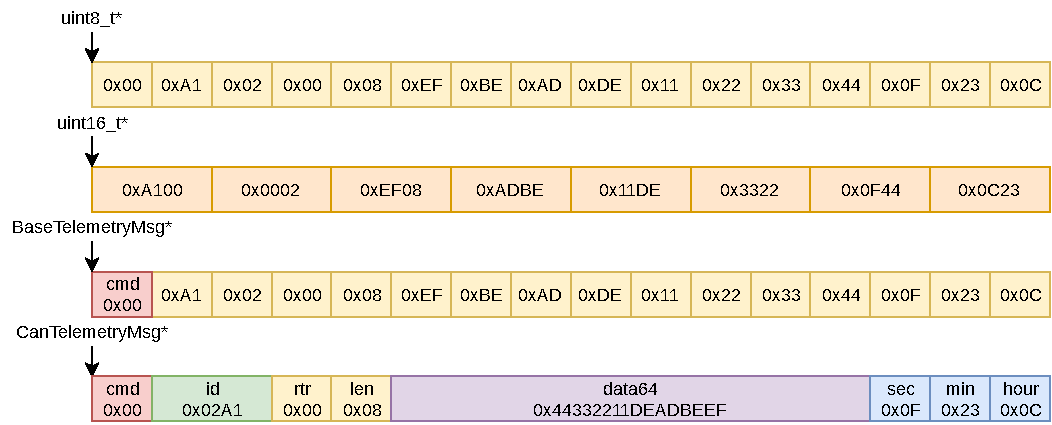
\includegraphics[width=\linewidth]{documentation/images/MessageTypes.pdf}
    \caption{The different message types used in the telemetry system.\todo{delete uint16\_t part in fig and make cmd to broadcast can}}
    \label{fig:messageTypes}
\end{figure}

\todo{make clearer distinction between message types and commands. Several commands can share the same message type}

The first byte, the command, always identifies the message type and indicates how the remaining 15 bytes should be interpreted. This eases the decoding of messages on the receiving end and makes for a expandable framework which has enough room for future expansions. 

As an example of a specific message type, figure \ref{fig:messageTypes} shows a message at the bottom with the command \texttt{BROADCAST\_CAN} which is encoded by \texttt{0x01}. This message carries a CAN message as a payload and commands the solar car subsystem to inject the message into the solar car CAN bus. Even though some message types are only sent one direction between the telemetry modules, a unified design was chosen due to the inherent simplicity.



% message protcol
% command system
% security -> encryption


\section{\todo{Final product}}
\subsection{Solar Car}
% threads 
\subsection{Support Vehicle}
% threads
\subsection{\todo{Graphical User Interface}}
% GUI 


\subsection{Components}
The primary components for our project has been two Teensy boards, a Teensy 3.6 board and 4.0 board, two nRF24 antennas, and a CAN transceiver. These components make up the chain of communication from reading/writing data from/to the CAN bus, through the Teensy boards CAN ports, to the antenna for transmission to the other antenna and Teensy board.

In addition to these components, we have used a 12V to 5V DC converter, a logic converter from 5V to 3V, a molex board connector, a 100\(\mu\)F capacitor, a coin cell battery holder and a perf board for implementing our solution with the above mentioned components. We have also made use of Arduino Uno boards during the development to generate random CAN data.

\subsection{Software Stack}

In this section the main software tools and libraries used throughout the project are introduced.

\subsubsection{PlatformIO}


\subsubsection{ChibiOS}
An open-source RTOS for embedded systems including Teensy. It supports threads, semaphores, data-sharing and timers and more to ease the scheduling of different tasks by the program kernel. 

\subsubsection{ACAN}
The ACAN library by Pierre Molinaro is a CAN network driver for the Teensy 3.6 board, as well as older Teensy series 3 boards. The library has been important for the connection between the CAN network and the ports on the Teensy board. We have only used the classic CAN configuration, but in addition to this, the library supports Flex CAN and CANFD. The driver supports bit rates ranging from 62.5 kbit/s up to 1 Mbit/s\cite{ACAN}.

\subsubsection{Other Libraries}

\subsection{CAN} % Victor
The CAN network in the solar car enables the micro-controllers at each electrical unit in the car to send and receive data without a host computer. This is possible with the special structure of the CAN message.

\begin{figure}[h]
    %\centering
    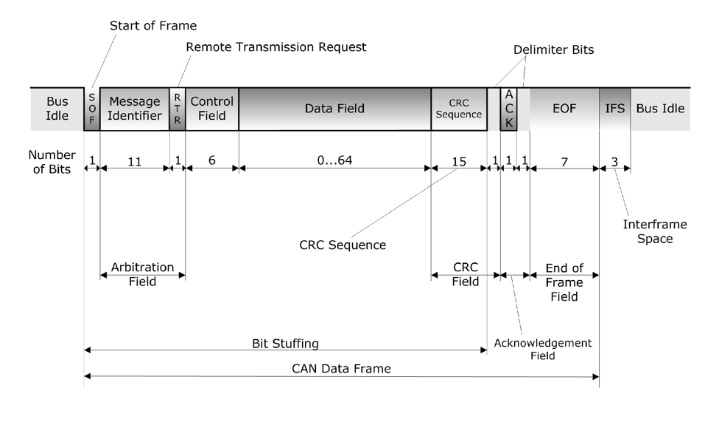
\includegraphics[scale=0.35]{documentation/images/detailed-can-data-frame-architecture.jpg}
    \caption{Structure of a CAN frame}
    \label{fig:CANframe}
\end{figure}

The frame uses an identifier to tell which messages goes to which unit. When two messages tries to access the bus, the one with the highest priority, lowest ID, will be granted access to the bus, while the other message has to wait. After the ID comes the RTR bit which determines whether the frame is set to be at sent or received by the node. The control field, sometimes called DLC, tells the amount of bytes used in the following frame field with actual data. The rest of the fields in fig. \ref{fig:CANframe} is not important concerning the nodes ability to communicate across the CAN network.

The CAN bus itself is two twisted wires, CAN High and CAN Low. These control the bits in the CAN message by setting a dominant and recessive voltage, which corresponds to a 0 and 1 respectively. A 1 is seen when the voltage in both wires is 2.5V while a 0 is seen when the CAN High wire is driven by 3.5V and the CAN Low wire is driven at 2.5V. 

Since the most transmitted message in the telemetry system will be CAN messages forwarded from the solar cars CAN bus, it is chosen to build the message protocol around 16 byte packets... \todo{talk about cmd and message types and more}\\
\todo{Should encryption be included in message protocol or a separate subsection?}
As an extra feature not included in our original specification, we have made an encryption protocol for our telemetry module. The encryption is based on the RSA encryption method, which essentially generates an encryption key based on the modulus and totient function of two prime numbers. When the message is encrypted, the type is converted from a unsigned 8-bit integer to an unsigned 16-bit integer, to avoid overflow problems. The encrypted message is then decrypted at the other module and converted back to unsigned 8-bit type. This effectively halves the amount of data we can send in our transmissions, which is the downside of our encryption solution.\\
The combinations of two prime numbers suited for the encryption protocol can be seen in the below table, 



\section{Implementation}

\subsection{Solar Car} 
\subsubsection{Black Box} % tjark

The black box functionality in the solar car is implemented using a SD card. The Teensy 3.6 used as a microcontroller in the telemetry module of the solar car already includes a 4-bit 

\subsubsection{CAN transceiver}
\subsection{Support Vehicle}
\subsubsection{GUI} % tjark
\subsubsection{RF transceiver}

\section{Verification and validation} % Victor
As mentioned in the methodology section, we spent time thoroughly verifying and validating our code design. We undertook the software verification after finishing the prototype and software coding, reviewing the naming, functionality and commenting the code accordingly.

We performed software validation as we went along with the software coding, to make sure that the actual behaviour of the code was as the expected behaviour. This was done through the testing environment in PlatformIO. We used this to validate our code design with unit tests, testing both edge cases and random cases. We chose only to validate the code and functions we made ourselves, and not those that was imported from external libraries.

Doing this provided us a test bench for our project, which greatly improved the credibility of our work, proving that our design works in general cases and not just the case we represent in our report.

\section{Discussion}
% variable length messages would reduce overhead -> but most messages contain CAN and are optimized
% 

\section{Conclusion}
The conclusion goes here.



\section*{Acknowledgment}
The authors would like to thank Martin Schoeberl and Christian Kampp Kruse for their mentoring and assistance throughout the project. The authors would also like to thank Claus Suldrup Nielsen from the department of Mechanical Engineering at DTU.


\printbibliography

\end{document}
